\chapter{닫힌 끈, 레벨 매칭과 쌍대성}

\lectureoverview{닫힌 끈에서는 끈의 두 내재적 방향을 따라 독립적인 파동이 생긴다. 이 파동들을 양자화하면 처음에는 열린 끈의 광자가 두 배로 늘어나는 듯하지만, 끈 좌표의 원점을 옮기는 변환에 대한 불변성이 한쪽 방향에만 있는 상태들을 제거한다. 처음으로 남는 레벨에는 질량이 없는 스핀 2 입자가 들어 있다. 기술 방식을 바꾼다는 같은 발상은 더 넓은 질문으로 이어진다. 결합이 변할 때 무엇을 근본적인 대상이라고 해야 할까?}

\section{남겨 둔 생성자}

닫힌 끈을 그리기 전에 정준역학에서 사실 하나를 다시 살펴보자. 다음과 같이 두고
\begin{equation}
  L=L(q_i,\dot q_i),
\end{equation}
\(q_i\)에 켤레인 운동량을 다음과 같이 정의하자.
\begin{equation}
  p_i=\frac{\partial L}{\partial\dot q_i}.
\end{equation}
무한소 연속 변환은 다음과 같이 쓸 수 있다.
\begin{equation}
  \delta q_i=\epsilon f_i(q),
  \label{eq:l04-infinitesimal-transformation}
\end{equation}
여기서 \(\epsilon\)은 작은 매개변수다. 이 변환이 대칭 변환이면 뇌터 정리에 따라 보존 전하가 주어진다. 좌표 변위를 공통 매개변수로 나누면 생성자는 다음과 같다.
\begin{equation}
  Q=\sum_i p_i f_i(q)
   =\frac{1}{\epsilon}\sum_i p_i\,\delta q_i.
  \label{eq:l04-noether-charge}
\end{equation}
양자역학에서 \(Q\)는 이에 대응하는 무한소 변환을 생성하는 연산자다.

\(xy\) 평면에서의 회전이 익숙한 예다. 방향을 한 가지로 정하면,
\begin{equation}
  \delta x=\epsilon y,
  \qquad
  \delta y=-\epsilon x,
\end{equation}
\eqref{eq:l04-noether-charge}은 같은 부호 선택에 따라 각운동량이 된다. 여기서는 이 구체적인 예가 중요하지 않다. 중요한 것은 운동량과 무한소 변위를 축약해 얻는 것이 생성자라는 관계다.

\begin{figure}[H]
  \centering
  \includegraphics[width=0.76\textwidth]{lecture_04_figure_01.png}
  \caption{나중에 닫힌 끈 좌표를 옮기는 변환에 쓸 정준 운동량과 뇌터 생성자.}
  \lectureframe{00:05:00}
  \label{fig:l04-noether-board}
\end{figure}

곧 우리가 마주할 대칭의 좌표는 보통 공간의 한 점이 아니라 끈을 따라 점들에 붙인 표지다. 식 \eqref{eq:l04-noether-charge}을 바로 활용할 수 있도록 여기서 다시 살펴보았다.

\section{고리를 따라 정의한 좌표}

닫힌 끈에는 끝점이 없다. 매개변수
\begin{equation}
  0\leq \sigma<2\pi
\end{equation}
를 택하고, 일단 한 점을 \(\sigma=0\)로 표시하자. 한 바퀴의 절반 지점은
\(\sigma=\pi\)이고, 사분의 일 바퀴와 사분의 삼 바퀴 지점은 각각 \(\pi/2\)와
\(3\pi/2\)이다. 이 표시는 좌표 규약을 정할 뿐, 아직 물리적 특징을 나타내지는 않는다.

\begin{figure}[H]
  \centering
  \begin{minipage}[t]{0.58\textwidth}
    \centering
    \includegraphics[width=\textwidth]{lecture_04_figure_02.png}
    \par\smallskip\footnotesize (a) 칠판에 그린 표식 있는 고리.
  \end{minipage}\hfill
  \begin{minipage}[t]{0.37\textwidth}
    \centering
    \begin{adjustbox}{max width=\linewidth}
    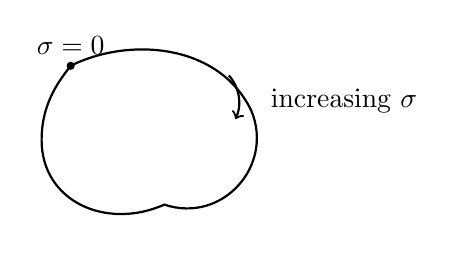
\begin{tikzpicture}[scale=0.82]
      \draw[thick]
        (0.1,1.1)
        .. controls (1.0,1.55) and (2.4,1.45) .. (2.9,0.4)
        .. controls (3.25,-0.45) and (2.45,-1.35) .. (1.55,-1.05)
        .. controls (0.65,-1.45) and (-0.35,-1.0) .. (-0.35,-0.05)
        .. controls (-0.35,0.55) and (-0.05,0.9) .. (0.1,1.1);
      \fill (0.1,1.1) circle (1.8pt);
      \node[above] at (0.1,1.12) {\(\sigma=0\)};
      \draw[->,thick] (2.55,0.95) arc[start angle=42,end angle=-25,radius=0.62];
      \node[right] at (3.05,0.55) {increasing \(\sigma\)};
    \end{tikzpicture}
    \end{adjustbox}
    \par\smallskip\footnotesize (b) 내재적 방향.
  \end{minipage}
  \caption{원점을 정하기 위해 한 점을 표시하고, 화살표로 \(\sigma\)가 증가하는 방향을 정한다.}
  \lectureframe{00:06:48}
  \label{fig:l04-closed-string-origin}
\end{figure}

고리를 따라 그은 화살표는 \emph{내재적} 방향이다. 이를 \(xy\) 평면에서 시계 방향 또는 반시계 방향으로 움직이는 것과 혼동해서는 안 된다. 표식이 있는 고무 밴드를 칠판에서 들어 뒤집은 다음 다시 놓는다고 생각해 보자. 겉으로 보이는 시계 방향은 반대로 바뀌지만, 밴드에 찍힌 표식의 내재적 순서는 바뀌지 않는다. \(\sigma\)가 증가하는 방향은 여전히 \(\sigma\)가 증가하는 방향이다.

이 구분은 오른쪽 진행파와 왼쪽 진행파라는 표현의 뜻을 결정한다. 이 장에서 오른쪽 진행 교란은 \(\sigma\)가 증가하는 쪽으로 진행하는 교란을 뜻하고, 왼쪽 진행 교란은 \(\sigma\)가 감소하는 쪽으로 진행하는 교란을 뜻한다. 어느 표현도 교란이 방 안에서 어느 쪽으로 움직여 보이는지를 말해 주지는 않는다.

방향성은 원래 강입자 끈 모형에서 구체적인 역할을 했다. 방향이 정해진 플럭스 튜브가 끊어지면 한쪽 끝에는 쿼크가, 다른 쪽 끝에는 반쿼크가 생기며, 내재적 화살표가 두 끝을 구별한다. 무방향 끈 이론도 구성할 수 있지만, 여기서는 화살표와 그에 따른 두 진행 방향을 유지한다.

\section{주기성과 진행파}

\(X(\sigma,\tau)\)과 \(Y(\sigma,\tau)\)를 끈의 두 횡방향 좌표라 하고, \(\tau\)는 시간을 나타낸다고 하자. 횡방향 좌표가 더 있는 경우에도 똑같이 다룬다. \(\sigma=0\)과 \(\sigma=2\pi\)은 같은 점을 나타내므로,
\begin{equation}
  X(\sigma+2\pi,\tau)=X(\sigma,\tau),
  \qquad
  Y(\sigma+2\pi,\tau)=Y(\sigma,\tau).
  \label{eq:l04-periodicity}
\end{equation}

\begin{figure}[H]
  \centering
  \includegraphics[width=0.76\textwidth]{lecture_04_figure_03.png}
  \caption{두 횡방향 좌표에 대한 주기 경계 조건.}
  \lectureframe{00:12:40}
  \label{fig:l04-periodicity-board}
\end{figure}

따라서 국소적으로 생긴 물결은 끝없이 순환할 수 있다. 물결이 \(2\pi\)에 도달하면 \(0\)에 다시 나타난다. 진행파가 끝점에 도달해 반사되고, 왼쪽 진행파가 오른쪽 진행파로 또는 그 반대로 바뀌는 열린 끈의 경우와 다르다. 열린 끈에서는 정상파가 자연스럽지만, 닫힌 끈에서는 서로 독립적으로 전파되는 두 계열이 가능하다.

\subsection{복소 푸리에 모드}

주기함수에 편리한 기저는 다음과 같다.
\begin{equation}
  e^{in\sigma}=\cos(n\sigma)+i\sin(n\sigma),
  \qquad n\in\mathbb Z.
\end{equation}
주기성 때문에 지수는 정수여야 한다.
\(e^{in(\sigma+2\pi)}=e^{in\sigma}\)예를 들어 \(n\)를 반정수로 바꾸면 한 바퀴 돈 뒤 함수가 처음 값으로 돌아오지 않는다.

시간 의존성을 잠시 생략하면, 칠판의 전개는 다음과 같다.
\begin{align}
  X(\sigma)
  &=
  X_0+
  \sum_{n>0}X_n e^{in\sigma}
  +\sum_{n>0}X_{-n}e^{-in\sigma},
  \label{eq:l04-fourier-x}\\
  Y(\sigma)
  &=
  Y_0+
  \sum_{n>0}Y_n e^{in\sigma}
  +\sum_{n>0}Y_{-n}e^{-in\sigma}.
  \label{eq:l04-fourier-y}
\end{align}
고전적인 수준에서 실수 \(X\)와 \(Y\)의 음의 지수 계수는 양의 지수 계수의 복소켤레다. 영모드 \(X_0\)와 \(Y_0\)는 질량 중심의 위치를 나타내며, 내부 진동이 아니다.

\begin{figure}[H]
  \centering
  \includegraphics[width=0.82\textwidth]{lecture_04_figure_04.png}
  \caption{주기 푸리에 전개에서 양의 지수 항과 음의 지수 항을 쓴 다음 영모드를 더한다.}
  \lectureframe{00:20:00}
  \label{fig:l04-fourier-board}
\end{figure}

\begin{classroomqa}
\audiencequestion{이 파동들이 움직인다면 시간 좌표는 어디에 있나요?\lecturetimestamp{00:19:05}}
\lecturerresponse{칠판 표기에서만 시간을 생략했다. 진행파 해의 위상에는 \(\sigma\)와 \(\tau\)가 모두 들어간다. 아래에서 사용할 약속에 따르면 한 계열의 위상 인자는
\(e^{-in(\tau-\sigma)}\)이고, 다른 계열은
\(e^{-in(\tau+\sigma)}\)이다.}
\end{classroomqa}

따라서 전파 방향을 결정하는 것은 순전히 공간적인 푸리에 인자에서 \(n\)의 부호만 보는 것이 아니라 전체 위상을 보는 것이다. 다음과 같이 쓸 수 있다.
\begin{equation}
  X(\sigma,\tau)=X_R(\tau-\sigma)+X_L(\tau+\sigma),
  \label{eq:l04-chiral-solution}
\end{equation}
\(Y\)에 대해서도 마찬가지다. 어느 계열을 \(R\), 어느 계열을 \(L\)라 부르는지는 약속에 달려 있다. 변하지 않는 사실은 \(\sigma\) 원을 따라 서로 반대 방향인 두 진행 방향이 있다는 것이다.\editorialnote{\(e^{in\sigma}\)라는 인자만으로는 한 순간의 파동이 움직이는지 알 수 없다. 전파 방향은 시간 위상을 함께 지정해야 정해진다.}

\section{두 방향의 에너지}

국소적인 동역학은 열린 끈의 경우와 같다. 여기서 쓰는 단순화된 정규화에서는,
\begin{equation}
  L\propto
  \int_0^{2\pi}d\sigma\,
  \left[
    \dot X^2-X'^2+\dot Y^2-Y'^2
  \right],
  \label{eq:l04-string-lagrangian}
\end{equation}
점은 \(\partial_\tau\)에 대한 미분을, 프라임은 \(\partial_\sigma\)에 대한 미분을 나타낸다. 에너지의 운동 항과 탄성 항 사이에는 더하기 부호가 있다.
\begin{equation}
  E\propto
  \int_0^{2\pi}d\sigma\,
  \left[
    \dot X^2+X'^2+\dot Y^2+Y'^2
  \right].
  \label{eq:l04-string-energy}
\end{equation}
횡방향 좌표 각각에 대해,
\begin{equation}
  \dot X^2+X'^2
  =
  \frac12(\dot X+X')^2+
  \frac12(\dot X-X')^2.
  \label{eq:l04-energy-square-completion}
\end{equation}
교차항은 상쇄되어 원래의 운동 에너지와 기울기 에너지만 남는다.

\begin{figure}[H]
  \centering
  \includegraphics[width=0.82\textwidth]{lecture_04_figure_05.png}
  \caption{전체 에너지를 두 진행파 부문으로 다시 나누어 쓴 식.}
  \lectureframe{00:25:10}
  \label{fig:l04-energy-board}
\end{figure}

\(X_R(\tau-\sigma)\)이면 \(\dot X_R=-X_R'\)이고, \(X_L(\tau+\sigma)\)이면 \(\dot X_L=X_L'\)이다. 따라서 \eqref{eq:l04-energy-square-completion}의 두 제곱항은 두 카이랄 계열을 각각 분리해 낸다. 모든 횡방향 좌표를 포함해 다음과 같이 정의하자.
\begin{align}
  E_L&\propto
  \frac12\int_0^{2\pi}d\sigma
  \sum_I(\dot X^I+X^{I\prime})^2,\\
  E_R&\propto
  \frac12\int_0^{2\pi}d\sigma
  \sum_I(\dot X^I-X^{I\prime})^2.
  \label{eq:l04-left-right-energies}
\end{align}
그러면 \(E=E_L+E_R\)이다. 이 단계에서는 방정식이 선형이므로 두 부문의 파동은 산란 없이 서로 통과한다.

\subsection{진동자의 수가 두 배}

푸리에 급수를 \eqref{eq:l04-string-lagrangian}에 대입하면 0이 아닌 각 모드 계수는 조화 진동자가 된다. 진동수는 \(|n|\)에 비례하므로 파장이 짧을수록 진동수가 높고, 따라서 들뜸 에너지도 커진다. 열린 끈과 달리 양의 진동수마다 서로 독립적으로 전파되는 모드가 두 개씩 존재한다.

칠판에서는 \(X\) 편광 생성 연산자를 \(a_n^+\)와 \(a_{-n}^+\)로, \(Y\) 편광 생성 연산자를 \(b_n^+\)와 \(b_{-n}^+\)로 표기한다. 생성과 전파를 더 명확히 구분하기 위해 다음 표기를 쓰겠다.
\begin{equation}
  a_n^\dagger,\quad b_n^\dagger,
  \qquad
  \widetilde a_n^\dagger,\quad\widetilde b_n^\dagger,
  \qquad n>0.
  \label{eq:l04-oscillator-notation}
\end{equation}
틸드가 없는 연산자와 틸드가 있는 연산자는 서로 반대인 세계면 방향의 진동자를 생성한다. \(a\)와 \(b\)는 두 횡방향 편광을 나타낸다.

\begin{figure}[H]
  \centering
  \includegraphics[width=0.65\textwidth]{lecture_04_figure_06.png}
  \caption{두 배가 된 \(X\) 편광 및 \(Y\) 편광 생성 연산자의 칠판 표기.}
  \lectureframe{00:29:10}
  \label{fig:l04-oscillators-board}
\end{figure}

\(N_n^{(a)},N_n^{(b)}\)와 그 틸드 동반 연산자가 점유수라면, 두 방향에 실리는 진동자 레벨은 개략적으로 다음과 같다.
\begin{equation}
  \begin{aligned}
    N&=\sum_{n>0}n\bigl(N_n^{(a)}+N_n^{(b)}+\cdots\bigr),\\
    \widetilde N&=\sum_{n>0}n
      \bigl(\widetilde N_n^{(a)}+\widetilde N_n^{(b)}+\cdots\bigr).
  \end{aligned}
  \label{eq:l04-level-operators}
\end{equation}
생략 부호는 다른 횡방향을 더 포함한다는 뜻이다.

\section{실패하는 스펙트럼 추측}

열린 끈의 첫 레벨을 떠올려 보자. 바닥 상태에 \(a_1^\dagger\) 또는 \(b_1^\dagger\)를 작용시키면 두 선형 편광을 얻는다. 이들의 원편광 조합은
\begin{equation}
  c_\pm^\dagger
  =
  \frac{1}{\sqrt2}
  \left(a_1^\dagger\pm i b_1^\dagger\right),
  \label{eq:l04-open-circular}
\end{equation}
헬리시티 \(h=\pm1\)를 갖는다. 헬리시티 0인 짝이 없다는 점은 이 기본적인 4차원 기술에서 질량 없는 벡터임을 나타낸다.

닫힌 끈의 바닥 상태 질량 제곱을 \(m_0^2\)라 하자. 가장 먼저 떠올릴 수 있는 단순한 추측은 다음 연산자 가운데 하나를 한 번 작용시키는 것이다.
\begin{equation}
  a_1^\dagger,\quad b_1^\dagger,\quad
  \widetilde a_1^\dagger,\quad\widetilde b_1^\dagger.
  \label{eq:l04-naive-one-sided}
\end{equation}
이는 전파 방향마다 하나씩, 열린 끈 광자가 두 사본 있는 경우와 비슷하다. 하지만 다음 에너지에서는 제한 없이 나열한 상태들이 타당한 회전 다중항을 이루지 못한다. 더 정교하게 분류해도 문제는 해결되지 않는다. 모든 진동자 단항식이 물리적 상태라는 전제가 잘못된 것이다.

\subsection{규칙으로 먼저 제시하는 레벨 매칭}

닫힌 끈의 물리적 조건은 다음과 같다.
\begin{equation}
  N=\widetilde N,
  \qquad\text{equivalently}\qquad E_L=E_R.
  \label{eq:l04-level-matching}
\end{equation}
우선 이 조건을 가정하자. 이 조건의 기원은 무엇을 이루는지 확인한 뒤에야 유도한다.

\eqref{eq:l04-naive-one-sided}의 모든 상태는 한 부문에는 에너지 한 단위가 있고 다른 부문에는 없으므로 전부 제외된다. 처음으로 살아남는 상태에는 각 계열에서 진동자가 하나씩 들어 있다.
\begin{align}
  a_1^\dagger\widetilde a_1^\dagger\ket{0},
  &\qquad
  b_1^\dagger\widetilde b_1^\dagger\ket{0},
  \label{eq:l04-four-matched-a}\\
  a_1^\dagger\widetilde b_1^\dagger\ket{0},
  &\qquad
  b_1^\dagger\widetilde a_1^\dagger\ket{0}.
  \label{eq:l04-four-matched-b}
\end{align}
이 상태들의 진동자 에너지는 총 2이며, 두 방향에 똑같이 나뉜다. \(n=2\) 생성 연산자 하나도 진동자 에너지 총량은 같지만 \eqref{eq:l04-level-matching}을 만족하지 않는다. 한쪽에만 에너지 두 단위를 보태기 때문이다.

\begin{figure}[H]
  \centering
  \includegraphics[width=0.70\textwidth]{lecture_04_figure_07.png}
  \caption{레벨 매칭을 만족하는 첫 레벨의 네 상태. 칠판에서는 \(1\)와 \(-1\)를 아래첨자로 쓰지만, \eqref{eq:l04-four-matched-a}--\eqref{eq:l04-four-matched-b}에서는 틸드가 없는 연산자와 틸드가 있는 연산자를 사용한다.}
  \lectureframe{00:41:05}
  \label{fig:l04-level-matched-board}
\end{figure}

\section{처음으로 매칭되는 레벨의 중력자}

두 카이랄 계열을 원편광 기저로 쓰면,
\begin{equation}
  c_\pm^\dagger
  =\frac{a_1^\dagger\pm i b_1^\dagger}{\sqrt2},
  \qquad
  \widetilde c_\pm^\dagger
  =\frac{\widetilde a_1^\dagger\pm i\widetilde b_1^\dagger}{\sqrt2}.
  \label{eq:l04-closed-circular}
\end{equation}
각 인자는 보통의 횡방향 공간에서 헬리시티 \(+1\) 또는 \(-1\)를 기여한다. 따라서 두 인자의 곱은 다음과 같다.
\begin{center}
\begin{tabular}{c c}
  \toprule
  상태 & 헬리시티 \\
  \midrule
  \(c_+^\dagger\widetilde c_+^\dagger\ket0\) & \(+2\) \\
  \(c_-^\dagger\widetilde c_-^\dagger\ket0\) & \(-2\) \\
  \(c_+^\dagger\widetilde c_-^\dagger\ket0\) & \(0\) \\
  \(c_-^\dagger\widetilde c_+^\dagger\ket0\) & \(0\) \\
  \bottomrule
\end{tabular}
\end{center}

\begin{classroomqa}
\audiencequestion{두 번째 원편광 인자는 반대 전파 부문에서 와야 하나요?\lecturetimestamp{00:43:20}}
\lecturerresponse{그렇다. 칠판에 처음 쓴 식은 바로 이 점 때문에 수정했다. 여기서 물리적 상태가 되려면 오른쪽 진행 진동자 하나와 왼쪽 진행 진동자 하나를 짝지어야 한다. 그렇지 않으면 레벨 매칭이 되지 않는다. 헬리시티는 횡방향 공간의 편광을 가리키며, 두 인자는 서로 반대인 세계면 방향을 가리킨다.}
\end{classroomqa}

\begin{figure}[H]
  \centering
  \includegraphics[width=0.82\textwidth]{lecture_04_figure_08.png}
  \caption{칠판 수정 뒤 원편광 기저로 쓴 네 곱과 각 헬리시티 \(+2,-2,0,0\).}
  \lectureframe{00:46:10}
  \label{fig:l04-helicity-board}
\end{figure}

질량을 가진 스핀 2 입자에는 스핀 투영값이 다섯 개 있다.
\begin{equation}
  m=2,1,0,-1,-2.
\end{equation}
매칭된 레벨에는 \(m=\pm1\)인 상태가 없다. 따라서 이 레벨은 질량을 가진 스핀 2 다중항일 수 없다. 반면 질량 없는 스핀 2 입자에는 헬리시티 \(+2\)와 \(-2\)만 있다. 같은 헬리시티를 곱해 얻는 두 상태가 바로 그 상태들이며, 중력자의 편광이다.

헬리시티 0인 조합이 두 개 더 남는다. 수업에서 사용한 표현으로 하나는 딜라톤이고 다른 하나는 악시온이다. 일반적인 닫힌 보존 끈의 공변적 기술에서는 이 설명을 더 세분한다.
\begin{equation}
  \begin{aligned}
    \alpha_{-1}^{I}\widetilde\alpha_{-1}^{J}\ket{0;k}
    &\longrightarrow
    \underbrace{h_{IJ}}_{\text{symmetric traceless}}
    \oplus
    \underbrace{B_{IJ}}_{\text{antisymmetric}}\\
    &\hspace{2.5em}\oplus
    \underbrace{\Phi}_{\text{trace}}.
  \end{aligned}
  \label{eq:l04-massless-tensor-decomposition}
\end{equation}
이들은 중력자, 반대칭 2-형식, 딜라톤이다. 4차원에서는 2-형식을 쌍대화해 악시온형 의사스칼라로 나타낼 수 있으며, 강의에서는 이 표현을 사용한다.\editorialnote{두 번째 헬리시티 0 상태의 본질은 일반적인 닫힌 끈 스펙트럼에 들어 있는 반대칭 텐서장 \(B_{\mu\nu}\)이다. 이를 악시온이라 부르는 것은 4차원에서의 쌍대 기술이다.}

이 형식적 수준에서는 세 장 모두 질량이 없다. 그러나 콤팩트화, 사영, 배경의 동역학에 따라 가벼운 상태로 남는 스칼라 또는 2-형식 자유도는 달라질 수 있다. 중력자는 다르다. 일관된 상호작용 닫힌 끈 부문이 있으면 그 안에 질량 없는 스핀 2 상태가 반드시 존재한다. 따라서 중력은 별도의 성분으로 덧붙이는 것이 아니라 닫힌 끈에서 나온다.

\section{레벨은 왜 매칭되어야 하는가}

이제 \(\sigma=0\)에 찍은 표식으로 돌아가자. 이것은 고리에 붙인 물리적 구슬인가, 아니면 매개변수의 원점일 뿐인가? 표식이 없는 보통의 닫힌 끈에서는 어느 점도 특별할 이유가 없다. 모든 표지를 함께 옮겨도 양자 상태는 변하지 않아야 한다.

\subsection{이산적인 경우}

고리를 횡방향 좌표 \((X_i,Y_i)\)가 붙은 순서 있는 점 \(M\)개로 이산화하자. 우선 \(Y_i\)는 생략한다. 배치 공간의 파동함수는 다음과 같다.
\begin{equation}
  \Psi(X_1,X_2,\ldots,X_M).
\end{equation}
첫 번째 점을 어디로 정하느냐를 바꾸면 순환 순열이 생긴다.
\begin{align}
  \Psi(X_1,X_2,\ldots,X_M)
  &=
  \Psi(X_2,\ldots,X_M,X_1)\nonumber\\
  &=
  \Psi(X_3,\ldots,X_M,X_1,X_2).
  \label{eq:l04-cyclic-wavefunction}
\end{align}
이것은 임의의 순열에 대한 불변성을 뜻하지 않는다. 예를 들어 \(X_1\)와 \(X_2\) 사이에 \(X_3\)를 끼워 넣으면 인접 관계가 바뀌어 이산화된 끈이 사실상 끊어졌다가 다시 연결된다. 선호되는 원점이 없음을 나타내는 것은 다음과 같은 공통 순환 재표지뿐이다.
\begin{equation}
  X_i\longrightarrow X_{i+1}\qquad(\text{mod }M)
  \label{eq:l04-discrete-shift}
\end{equation}

\begin{figure}[H]
  \centering
  \includegraphics[width=0.82\textwidth]{lecture_04_figure_09.png}
  \caption{이산화된 닫힌 끈의 순환 파동함수 항등식.}
  \lectureframe{00:56:20}
  \label{fig:l04-cyclic-board}
\end{figure}

\subsection{연속체에서의 표현}

연속체 극한 \(M\to\infty\)에서는 상태가 파동범함수로 주어진다.
\begin{equation*}
  \Psi[X(\sigma),Y(\sigma)].
\end{equation*}
순환 재표지는 다음과 같이 바뀐다.
\begin{equation}
  \sigma\longrightarrow\sigma+\epsilon.
\end{equation}
불변성은 다음을 뜻한다.
\begin{equation}
  \Psi[X(\sigma+\epsilon),Y(\sigma+\epsilon)]
  =
  \Psi[X(\sigma),Y(\sigma)].
  \label{eq:l04-wavefunctional-invariance}
\end{equation}

\begin{figure}[H]
  \centering
  \includegraphics[width=0.72\textwidth]{lecture_04_figure_10.png}
  \caption{이산적인 이동과 이에 대응하는 파동범함수의 연속체 표현.}
  \lectureframe{00:58:40}
  \label{fig:l04-wavefunctional-board}
\end{figure}

1차까지 전개하면,
\begin{equation}
  \delta X(\sigma)=\epsilon X'(\sigma),
  \qquad
  \delta Y(\sigma)=\epsilon Y'(\sigma),
  \label{eq:l04-profile-shift}
\end{equation}
프로필의 능동적 이동과 좌표의 수동적 이동을 구분하는 전체 부호는 제외했다. 이에 대응하는 파동범함수의 변분은 다음과 같다.
\begin{equation}
  \delta\Psi
  =
  \epsilon\int_0^{2\pi}d\sigma
  \left[
    \frac{\delta\Psi}{\delta X(\sigma)}X'(\sigma)
    +
    \frac{\delta\Psi}{\delta Y(\sigma)}Y'(\sigma)
  \right].
  \label{eq:l04-functional-variation}
\end{equation}

\begin{figure}[H]
  \centering
  \includegraphics[width=0.72\textwidth]{lecture_04_figure_11.png}
  \caption{이동된 파동범함수 인자의 1차 전개.}
  \lectureframe{01:01:31}
  \label{fig:l04-functional-expansion-board}
\end{figure}

\begin{classroomqa}
\audiencequestion{1차 조건은 \(\sigma\)의 각 값마다 별도의 방정식인가요?\lecturetimestamp{01:01:30}}
\lecturerresponse{아니다. 이 변환은 끈의 모든 점을 함께 옮긴다. 한 점에서의 변분을 다른 모든 점에서의 변분과 더해야 하므로 연속체 표현에 \(\sigma\)에 대한 적분이 들어간다.}
\end{classroomqa}

좌표 표현에서는,
\begin{equation}
  P_X(\sigma)=-i\frac{\delta}{\delta X(\sigma)},
  \qquad
  P_Y(\sigma)=-i\frac{\delta}{\delta Y(\sigma)}
  \label{eq:l04-functional-momenta}
\end{equation}
\(\hbar=1\)일 때다. 따라서 식 \eqref{eq:l04-functional-variation}은 다음 생성자에 의해 만들어진다.
\begin{equation}
  G_\sigma=
  \int_0^{2\pi}d\sigma\,
  \left[
    P_X(\sigma)X'(\sigma)+P_Y(\sigma)Y'(\sigma)
  \right].
  \label{eq:l04-sigma-generator}
\end{equation}
이는 뇌터 관계 \eqref{eq:l04-noether-charge}와 정확히 같다. 즉 모든 자유도에 대해 정준 운동량에 좌표 변위를 곱해 합한 것이다. 표식이 없는 닫힌 끈의 상태는 다음을 만족한다.
\begin{equation}
  G_\sigma\ket{\mathrm{phys}}=0.
  \label{eq:l04-physical-generator-condition}
\end{equation}

\eqref{eq:l04-string-lagrangian}의 정규화에서는,
\(P_I\propto\dot X^I\)이므로 같은 조건을 다음과 같이 쓸 수 있다.
\begin{equation}
  \int_0^{2\pi}d\sigma
  \sum_I\dot X^I X^{I\prime}=0.
  \label{eq:l04-momentum-constraint}
\end{equation}

\begin{figure}[H]
  \centering
  \includegraphics[width=0.75\textwidth]{lecture_04_figure_12.png}
  \caption{파동함수의 함수 미분을 운동량으로 놓은 뒤의 적분 생성자.}
  \lectureframe{01:05:10}
  \label{fig:l04-generator-board}
\end{figure}

\subsection{생성자는 에너지 차이다}

\eqref{eq:l04-left-right-energies}의 두 식을 더하면 전체 에너지가 되고, 빼면 다음과 같다.
\begin{align}
  E_L-E_R
  &\propto
  \frac12\int_0^{2\pi}d\sigma\sum_I
  \left[
    (\dot X^I+X^{I\prime})^2\right.\nonumber\\[-0.25em]
  &\hspace{7em}\left.
    -(\dot X^I-X^{I\prime})^2
  \right]\\
  &=
  2\int_0^{2\pi}d\sigma\sum_I
  \dot X^I X^{I\prime}.
  \label{eq:l04-energy-difference}
\end{align}
이 적분은 물리적 상태를 소멸시켜야 하는 생성자다. 따라서
\begin{equation}
  E_L-E_R=0,
  \qquad\text{or}\qquad
  N-\widetilde N=0.
\end{equation}
레벨 매칭이란 \(\sigma\) 좌표의 원점을 관측할 수 없다는 뜻이다.

\begin{figure}[H]
  \centering
  \includegraphics[width=0.78\textwidth]{lecture_04_figure_13.png}
  \caption{레벨 매칭 유도의 끝에서 함께 보인 에너지의 합과 차.}
  \lectureframe{01:06:40}
  \label{fig:l04-energy-difference-board}
\end{figure}

\begin{classroomqa}
\audiencequestion{표시된 식에서 절반 계수의 위치가 서로 다른 것처럼 보이는 이유는 무엇인가요?\lecturetimestamp{01:06:28}}
\lecturerresponse{여기서는 상대적인 구조만 사용합니다. 일관된 전체 정규화를 복원하면 완전제곱 항등식 \eqref{eq:l04-energy-square-completion}에 절반 계수가 나타납니다. 합은 전체 에너지를 주고, 차는 \(\int d\sigma\,\dot X X'\)에 비례한 채로 남습니다. 그 차이가 0이 되는 것, 따라서 레벨 매칭은 이 공통된 규약과 무관합니다.}
\end{classroomqa}

이 제약은 순진하게 얻은 진동자 스펙트럼의 상당 부분을 제거하며, 타당한 입자 다중항을 이루지 못했던 상태들을 정확히 없앤다. 열린 끈에는 이 제약이 적용되지 않으므로 열린 끈의 광자는 제거되지 않는다. 닫힌 끈에는 이 닫힌 고리 조건을 받는 독립적인 순환 부문 두 개가 있다. 닫힌 끈에서는 중력자, 딜라톤, 반대칭 텐서 또는 악시온형 상태, 그리고 더 높은 매칭 레벨이 남는다.
\editorialnote{공변적 끈 양자화에서 레벨 매칭은 세계면 제약계 가운데 하나인 영모드 조건 \(L_0-\widetilde L_0=0\)이다. 여기서의 유도는 그 직관적 기원, 즉 닫힌 끈을 따라 평행이동해도 불변이어야 한다는 점을 드러낸다.}

\section{왼쪽과 오른쪽의 두 가지 뜻}

이제 왼쪽과 오른쪽을 가리키는 표현은 서로 무관한 두 가지 뜻으로 쓰인다.
\begin{enumerate}
  \item \(X_R(\tau-\sigma)\)와 \(X_L(\tau+\sigma)\)는 내재적인 \(\sigma\) 원을 따라 서로 반대 방향으로 전파됨을 나타낸다.
  \item \(c_+^\dagger\)와 \(c_-^\dagger\)는 물리적인 횡방향 \(xy\) 평면의 원편광을 나타낸다.
\end{enumerate}
레벨 매칭된 중력자 상태에는 세계면의 각 진행 방향에서 진동자가 하나씩 들어간다. 그렇더라도 두 진동자는 시공간에서 같은 헬리시티를 가질 수 있어 \(h=+2\) 또는 \(h=-2\)을 만든다. 왼쪽과 오른쪽의 이 두 뜻을 혼동하면 실제로는 모순이 아닌 스펙트럼이 모순처럼 보인다.

\section{근본적이라는 것은 무슨 뜻인가?}

열린 끈과 닫힌 끈을 이 기본적인 수준에서 양자화하고 나면 자연스러운 질문이 남는다. 끈은 더 이상 나눌 수 없는 최종 구성 요소인가, 아니면 끈 자체도 다른 무언가로 이루어졌을 수 있는가?

\begin{classroomqa}
\audiencequestion{끈을 가장 근본적인 대상으로, 즉 그보다 더 작은 구성 요소가 없다고 여길 증거나 이유가 있나요?\lecturetimestamp{01:10:44}}
\lecturerresponse{매개변수와 무관하게 쓸 수 있는 유용한 답은 없다. 한 영역에서 기본적으로 보이는 자유도가 다른 영역에서는 무겁고 확장된, 겉보기에는 복합적인 대상으로 바뀔 수 있다. 근본적이라는 말은 고려 중인 결합에서 어떤 변수가 유용한 기술을 제공하는지를 나타낸다고 보는 편이 가장 좋다.}
\end{classroomqa}

전하와 자기 전하의 관계가 이 답을 가장 분명하게 보여 준다. 이론에 전기 전하 \(e\)와 자기 전하 \(g\)가 있다고 하자. 자기홀극에 붙은 관측 불가능한 디랙 끈 때문에 다음 조건이 필요하다.
\begin{equation}
  eg=2\pi n,
  \qquad n\in\mathbb Z.
  \label{eq:l04-dirac-quantization}
\end{equation}
최소 전하의 경우 \(n=1\)이다. 그러면 디랙 끈 주위를 도는 하전 입자는 위상 \(e^{ieg}=1\)를 얻으므로 보조적인 끈을 검출할 수 없다.

\begin{figure}[H]
  \centering
  \begin{minipage}[t]{0.58\textwidth}
    \centering
    \includegraphics[width=\textwidth]{lecture_04_figure_14.png}
    \par\smallskip\footnotesize (a) 칠판에 쓴 디랙 양자화 조건.
  \end{minipage}\hfill
  \begin{minipage}[t]{0.36\textwidth}
    \centering
    \begin{adjustbox}{max width=\linewidth}
    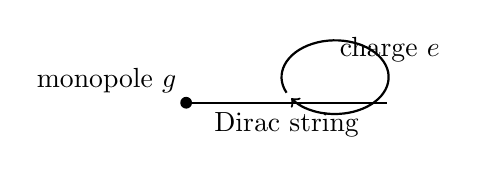
\begin{tikzpicture}[scale=0.85]
      \fill (0,0) circle (2.5pt);
      \node[above left] at (0,0) {monopole \(g\)};
      \draw[thick] (0,0) -- (3.0,0);
      \node[below] at (1.5,0) {Dirac string};
      \draw[->,thick] (1.5,0.15) arc[start angle=205,end angle=-145,
        x radius=0.8,y radius=0.55];
      \node[right] at (2.15,0.8) {charge \(e\)};
    \end{tikzpicture}
    \end{adjustbox}
    \par\smallskip\footnotesize (b) 끈 주위에서 위상을 측정하는 실험.
  \end{minipage}
  \caption{디랙 조건에 따라 전기 전하와 자기 전하는 서로 역수 관계를 이룬다.}
  \lectureframe{01:13:20}
  \label{fig:l04-dirac-board}
\end{figure}

\(e\)가 작으면 전기 변수로 전개하는 보통의 섭동론이 유용하다. 전기 꼭짓점이 추가된 파인만 도표의 기여는 점점 더 억제된다. 그러나 \eqref{eq:l04-dirac-quantization}에 따르면 \(g\)는 커지므로 자기 꼭짓점에 대한 도표 전개는 유용하지 않다. 보통의 무차원 결합으로 쓰면,
\begin{equation}
  \alpha_e=\frac{e^2}{4\pi},
  \qquad
  \alpha_m=\frac{g^2}{4\pi},
  \qquad
  \alpha_e\alpha_m=\frac{n^2}{4}.
  \label{eq:l04-dual-couplings}
\end{equation}
전기 결합이 약하면 자기 결합은 강하고, 그 반대도 성립한다.

전기적 기술에서 강하게 결합된 자기홀극은 복잡한 대상처럼 보이기도 한다. 장 에너지가 크고, 강한 게이지장 요동과 자기 전하를 띤 가상 쌍의 구름에 둘러싸여 있다. 무겁고 확장된 대상처럼 행동하므로 전기적 섭동 급수의 출발점으로는 적절하지 않다. 그렇다고 이 대상이 덜 근본적임을 증명하는 것은 아니다. 해당 영역을 기술하기에는 이 대상이 기본 변수가 아니라는 뜻이다.

이제 \(e\)를 연속적으로 증가시킨다고 하자. 양자화 조건 때문에 \(g\)는 감소한다. 자기쌍대 영역 근처에서는 어느 기술도 특별히 약결합이 아니며, 그 영역을 지나면 자기 변수가 더 단순하고 가벼운 변수가 될 수 있다. 반면 전기적 대상은 강하게 둘러싸인다. 어느 전하를 기본이라고 불러야 하는지는 달라졌지만 이론의 물리적 내용은 바뀌지 않았다.

\subsection{위그너의 질문}

힉스 보손이 근본적인지 복합적인지를 두고 논의하던 중 한때 이 모호함이 드러났다. 유진 위그너는 복합적이라는 말의 뜻을 거듭 물었다. 한 가지 구분 기준으로 붕괴 여부가 제안되었다. 어쩌면 근본적인 대상은 붕괴할 수 없고 복합적인 대상은 붕괴할 수 있다는 것이다. 하지만 바닥 상태인 수소 원자는 붕괴할 수 없으면서도 명백히 복합적이다. 양성자는 안정할 수 있고 중성자는 붕괴할 수 있지만, 의도된 의미에서 전자가 전자보다 더 기본적이라는 뜻은 아니다. 단순한 정의를 내놓을 때마다 또 다른 반례가 나왔다.

헤라르뒤스 토프트는 실용적인 기준을 제시하며 논의를 마무리했다. 어떤 대상을 근본적인 것으로 생각하는 것이 유용할 때 그 대상은 근본적이다. 이는 답을 회피하는 말이 아니다. 기본적이라는 말은 동역학이 단순해지는 변수를 가리키며, 단순성은 결합과 환경에 따라 달라질 수 있다는 점을 인정한 것이다.

\section{M이론을 향하여}

끈 이론에서는 역할의 교환이 특히 선명하게 나타난다. 한 매개변수 영역에서는 끈이 가볍고 섭동적으로 다루기 쉬운 반면, D-막은 끈 자유도로 이루어진 무거운 솔리톤 복합체처럼 보인다. 매개변수가 바뀌면 D-막이 더 가벼운 기본적 대상이 될 수 있고, 첫 번째 영역에서 끈으로 기술했던 배치를 D-막의 관점으로 다시 해석할 수 있다. 근본적으로 보이던 것이 복합적으로 바뀔 수 있고, 복합적으로 보이던 것이 근본적인 것으로 바뀔 수 있다.

오래된 환원주의적 관점은 큰 것에서 더 작은 구성 요소로, 마침내 유일한 바닥 층에 이르기까지 한 방향으로 내려가는 그림을 제시한다. 쌍대성은 그보다 덜 선형적인 그림을 시사한다. 결합이 변하면 기술 방식들이 서로 변환될 수 있으며, 어느 곳에서나 우선시되는 단일한 변수 집합은 없다. 다음 주제인 M이론은 이러한 관점에서 살펴볼 것이다.

보존 끈 이론의 임계 차원이 26이고 초끈 이론의 임계 차원이 10인 이유는 여기서 아직 해결되지 않은 문제로 남아 있다. 다음으로 넘어가기 전에 모든 기술적 문제를 해결하려 하기보다, 이제 관점을 바꾸어 적절한 극한에서 M이론이 어떻게 끈 이론을 만들어 낼 수 있는지 묻겠다.